% !TEX root = handbook-physics.tex
% !TEX TS-program = pdflatex
% !TEX encoding = UTF-8 Unicode






\chapter{Direct Electric Current}
\label{ch-21}
\zhtitle{直流电流}

\section{Extraneous Forces}
\label{sec-21.1}
\zhtitle{非静电力}

\subsection{}\label{21.1.1} 
 A metallic conductor has an electrostatic held that is set up by the electrons and positive ions of the crystal lattice. This is a held of Coulomb forces \ssect{14.2.2}. Coulomb interaction between the charges in a metal leads to such an equilibrium distribution of charges that the electric held inside the conductor equals zero and the whole conductor is equipotential \ssect{16.4.3}. Consequently, an electrostatic Coulomb held cannot be the cause of the steady-state process of ordered motion of electrons, i.e. it cannot generate and maintain a direct (constant) current. 
\zhpar{金属导体中存在由电子和晶格中的正离子所建立的静电场。这是库仑力场\ssect{14.2.2}。金属中电荷之间的库仑相互作用导致电荷达到这样的平衡分布：导体内部的电场为零，整个导体为等势体\ssect{16.4.3}。因此，静电库仑场不可能是电子有序运动这一稳恒过程的原因，即它无法产生并维持直流（恒定）电流。}
 
\subsection{}\label{21.1.2} \redem{Extraneous forces} are non-electrostatic forces whose action exerted on the conduction electrons in the conductor initiates their ordered motion and maintains a direct (constant) electric current in the circuit. In contrast to Coulomb forces, extraneous forces do not join unlike charges; they lead to their separation and maintain a potential difference at the ends of the conductor.
\zhpar{\redem{非静电力}是指这样一类非静电性质的力：它作用于导体中的传导电子，使其作有序运动，并在电路中维持直流（恒定）电流。与库仑力不同，非静电力不会使异号电荷相互靠拢，而是使它们分离，并在导体两端维持电势差。}

Extraneous forces are the cause of the non-electrostatic electric held, existing in the conductor and providing for ordered motion of the charges from points with a higher potential to points with a lower potential. A steady-state electric held of extraneous forces is set up by \redem{sources of electrical energy} (galvanic cells, electric generators, etc.).
\zhpar{非静电力是导体内部存在的非静电性电场的起因，该电场使电荷从高电势点向低电势点作有序运动。由非静电力建立的稳恒非静电电场由\redem{电源}（原电池、发电机等）产生。}

\begin{marginfigure}
\centering
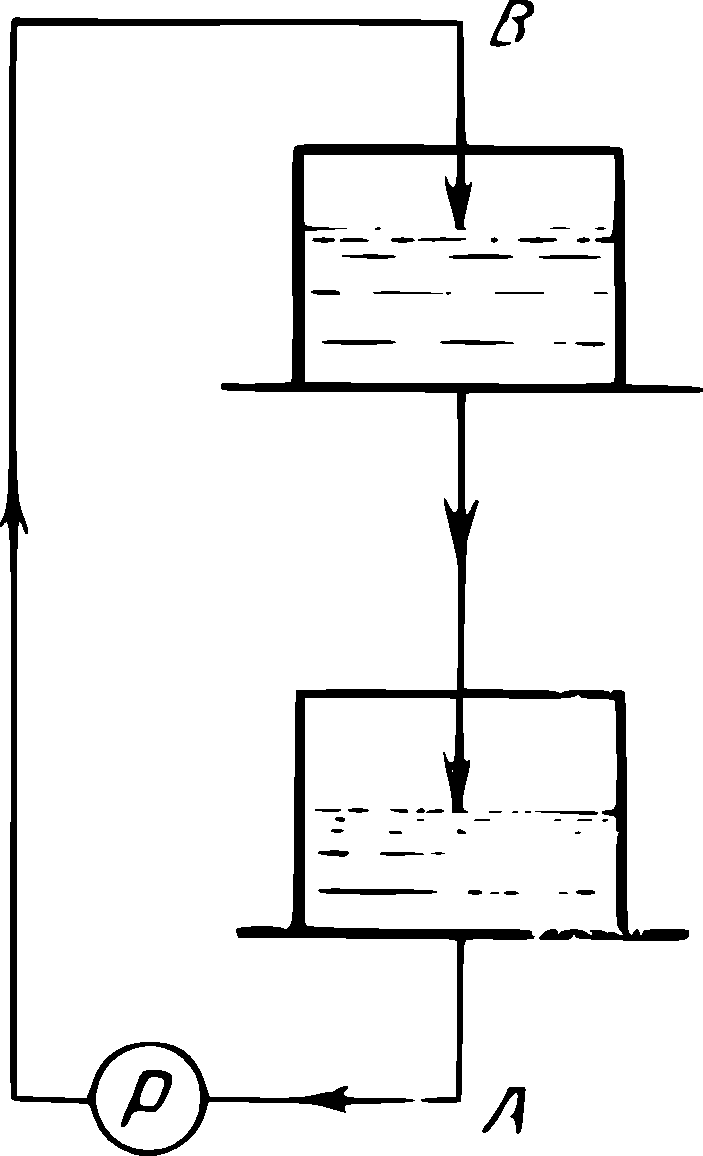
\includegraphics[width=0.7\textwidth]{figs/ch-21/fig-21-01.pdf}
\caption{An analogy of a hydraulic system for movement of charges.\zhcap{电荷运动的水力系统类比。}\label{fig-21-01}}
\end{marginfigure}

\subsection{}\label{21.1.3} In a closed hydraulic system maintaining constant liquid circulation (refer to (\figr{fig-21-01}), the liquid moves from point $A$ to point $B$ against the force of gravity due to the influence of external forces exerted by the pump $P$. The pump generates a consistent difference in hydrostatic pressure between points $B$ and $A$, prompting the liquid to flow against gravity from $B$ to $A$. A source of electrical energy plays a similar role in a direct current circuit. Owing to the electric field set up by extraneous forces and existing inside the source, the electric charges move within the source against the forces of the electrostatic field. This maintains a potential difference at the ends of the external circuit that is required for a direct current to flow. At the expense of the energy consumed in the source, work is done to obtain ordered motion of the electric charges.
\zhpar{在保持液体恒定循环的闭合水力系统中（见\figr{fig-21-01}），液体在泵 $P$ 施加的外力作用下，逆重力由点 $A$ 运动到点 $B$。泵在点 $B$ 与点 $A$ 之间产生稳定的静水压强差，促使液体逆重力从 $B$ 流向 $A$。在直流电路中，电源起着与之类似的作用。电源内部存在由非静电力建立的电场，电荷在电源内部逆着静电场的作用力运动，从而在外电路两端维持直流电流流动所需的电势差。电源内部所消耗的能量用于使电荷作有序运动而做功。}

In a direct current generator, for example, the work of the extraneous forces \ssect{21.1.2} is done at the expense of the mechanical energy required to drive the rotor of the generator.
\zhpar{例如，在直流发电机中，非静电力所做的功来源于驱动发电机转子所消耗的机械能。}

\section{Ohm's Law and the Joule-Lenz Law}
\label{sec-21.2}
\zhtitle{欧姆定律与焦耳-楞次定律}


\subsection{}\label{21.2.1} At any point inside a portion of a conductor that contains a source of electrical energy there is an electrostatic field of Coulomb forces with the strength $\vb{E}_{\text{Coul}}$ and an electric field of extraneous forces with the strength $\vb{E}_{\text{extr}}$.
\zhpar{在包含电源的一段导体内部的任一点，既存在场强为 $\vb{E}_{\text{Coul}}$ 的库仑力静电场，也存在场强为 $\vb{E}_{\text{extr}}$ 的非静电力电场。}

According to the principle of superposition of fields 
\ssect{15.2.2} the strength of the resultant field is
\zhpar{根据场的叠加原理\ssect{15.2.2}，合成场的场强为}
\begin{equation*}
\vb{E} = \vb{E}_{\text{Coul}} + \vb{E}_{\text{extr}}.
\end{equation*}
Ohm's law for current density \ssect{20.3.4},
\zhpar{由电流密度形式的欧姆定律\ssect{20.3.4}，}
\begin{equation*}
\vb{j} = \frac{1}{\rho} \, (\vb{E}_{\text{Coul}} + \vb{E}_{\text{extr}}),
\end{equation*}
enables the following relation to be obtained for portion 1-2 of a homogeneous conductor of cross-sectional area $S$:
\zhpar{由此可得到横截面积为 $S$ 的均匀导体上 1-2 段满足的如下关系：}
\begin{equation*}
I \int_{1}^{2} \rho \, \frac{\dd l}{S}  = \int_{1}^{2} \vb{E}_{\text{Coul}} \, \dd \vb{l} + \int_{1}^{2} \vb{E}_{\text{extr}} \, \dd \vb{l} ,
\end{equation*}
where $I$ is the current in the conductor, $\dd \vb{l}$ is a vector with the magnitude $\dd l$, equal to an element of conductor length, and is directed tangent to the conductor toward the current density vector, and $S$ is the cross-sectional area of the conductor.
\zhpar{式中 $I$ 为导体中的电流，$\dd \vb{l}$ 为导体长度的线元矢量，其大小为 $\dd l$，方向沿导体切线并指向电流密度矢量的方向；$S$ 为导体的横截面积。}


\subsection{}\label{21.2.2} 

The integral $\int_{1}^{2} \vb{E}_{\text{Coul}} \, \dd \vb{l} $ is numerically equal to the work done by the Coulomb forces in moving a unit positive charge from point 1 to point 2. According to \ssect{16.3.1}
\zhpar{积分 $\int_{1}^{2} \vb{E}_{\text{Coul}} \, \dd \vb{l}$ 在数值上等于库仑力把单位正电荷从点 1 移动到点 2 所做的功。根据\ssect{16.3.1}，}
\begin{equation*}
 \int_{1}^{2} \vb{E}_{\text{Coul}} \, \dd \vb{l}  = V_{1} - V_{2},
\end{equation*}
where $V_{1}$ and $V_{2}$ are the potentials at points 1 and 2 of the conductor.
\zhpar{其中 $V_{1}$ 和 $V_{2}$ 分别为导体上点 1 和点 2 处的电势。}

The \redem{electromotive force} (emf) $\emf_{12}$, acting over the portion 1-2 of the circuit, is the name given to the linear integral
\zhpar{作用于电路 1-2 段的\redem{电动势}（emf）$\emf_{12}$ 定义为下列线积分：}
\begin{equation*}
\emf_{12} = \int_{1}^{2} \vb{E}_{\text{extr}} \, \dd \vb{l}.
\end{equation*}
The electromotive force $\emf_{12}$ is numerically equal to the work done by the extraneous forces in moving a unit positive charge along the conductor from point 1 to point 2. This work is done at the expense of the energy consumed in the source.
\zhpar{电动势 $\emf_{12}$ 在数值上等于非静电力把单位正电荷沿导体从点 1 移动到点 2 所做的功。该功是消耗电源内部的能量而做的。}

The \redem{voltage} (or \redem{voltage drop}) $U_{12}$ across the portion 1-2 is the physical quantity numerically equal to the work done by the resultant field of Coulomb and extraneous forces in moving a unit positive charge along the circuit from point 1 to point 2. Thus
\zhpar{电路段 1-2 两端的\redem{电压}（或\redem{电压降}）$U_{12}$ 是一个物理量，其数值等于静电力与非静电力的合场把单位正电荷沿电路从点 1 移动到点 2 所做的功。于是有}
\begin{equation*}
U_{12}  = \int_{1}^{2} (\vb{E}_{\text{Coul}} + \vb{E}_{\text{extr}}) \, \dd \vb{l} = \int_{1}^{2} \vb{E} \, \dd \vb{l},
\end{equation*}
or
\zhpar{或写为}
\begin{equation*}
U_{12}  = (V_{1} - V_{2}) + \emf_{12}.
\end{equation*}
The voltage across the ends of the circuit coincides with the potential difference only when no emf is applied to this portion.
The integral
\zhpar{只有在该段电路中不存在电动势时，电路两端的电压才与电势差相等。下面的积分}
\begin{equation*}
R_{12} = \int_{1}^{2} \rho \, \frac{\dd \vb{l}}{S},
\end{equation*}
is the \redem{resistance} $R_{12}$ in the portion of the circuit between sections 1 and 2. For a homogeneous cylindrical conductor (wire), $\rho = \text{const}$, $S = \text{const}$ 
\zhpar{即为截面 1 与截面 2 之间这段电路的\redem{电阻} $R_{12}$。对于均匀圆柱形导体（导线），$\rho = \text{const}$，$S = \text{const}$，}
\begin{equation*}
R_{12} =  \rho \, \frac{l_{12}}{S},
\end{equation*}
where $l_{12}$ is the length of the conductor between cross sections 1 and 2.
\zhpar{其中 $l_{12}$ 为截面 1 与截面 2 之间导体的长度。}

\subsection{}\label{21.2.3} The generalized Ohm's law for an arbitrary portion of a circuit is
\zhpar{广义欧姆定律适用于电路中的任意一段，其形式为}
\begin{equation*}
I R_{12} = U_{12} = (V_{1} - V2)+ \emf_{12}.
\end{equation*}
The product of the current by the resistance of a portion of the circuit is equal to the potential difference across this portion plus the emf of all sources of electrical energy connected in the given portion of the circuit. In this form Ohm's law is applicable both for \redem{passive portions} of the circuit, not containing sources of electrical energy, as well as for \redem{active portions} that contain such sources.
\zhpar{一段电路中电流与该段电阻的乘积，等于该段两端的电势差与该段电路中所接全部电源的电动势之和。这一形式的欧姆定律既适用于不含电源的\redem{无源段}，也适用于含有电源的\redem{有源段}。}

\subsection{}\label{21.2.4} The \redem{sign rule} for the emf of sources of electrical energy included in portion 1-2 states that if the current inside the source is from the cathode to the anode, i.e. the strength of the field of extraneous forces coincides in direction with the current in this portion of the circuit, then, in calculations, the emf $\emf_{12}$ of this source is considered positive. If the current inside the source is from the anode to the cathode, the emf $\emf_{12}$ this source is considered negative (\figr{fig-21-02}).
\zhpar{对于电路段 1-2 中所接电源的电动势，采用如下\redem{符号规则}：若电源内部电流由阴极流向阳极，即非静电力电场的方向与该段电路中的电流方向一致，则计算时该电源的电动势 $\emf_{12}$ 取正值；若电源内部电流由阳极流向阴极，则该电源的电动势 $\emf_{12}$ 取负值（见\figr{fig-21-02}）。}

\begin{figure}
\centering
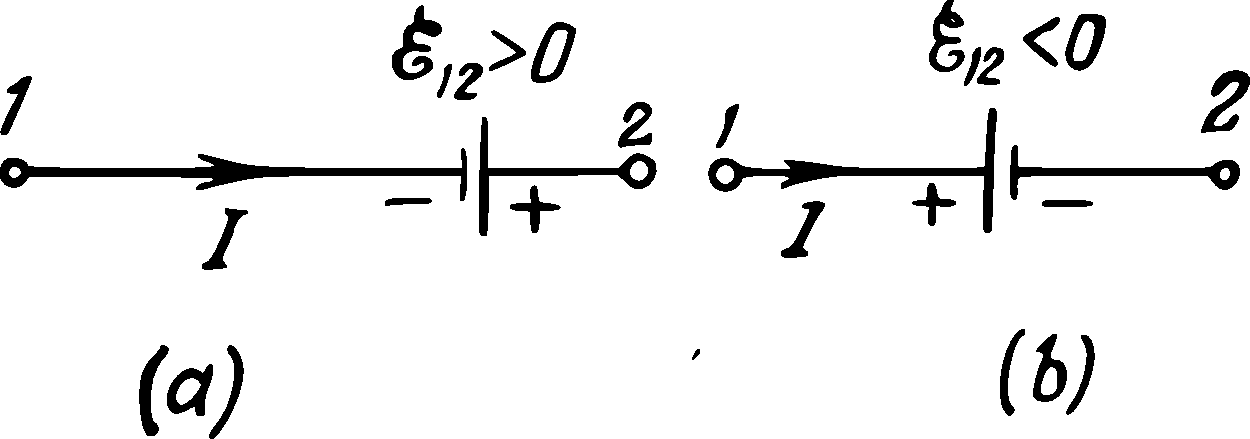
\includegraphics[width=0.7\textwidth]{figs/ch-21/fig-21-02.pdf}
\sidecaption{The sign rule for emf sources of electrical energy in a circuit.\zhcap{电路中电源电动势的符号规则。}\label{fig-21-02}}
\end{figure}


\subsection{}\label{21.2.5} In a closed series electric circuit, the current is the same at all cross sections, and such a circuit is a portion with coinciding ends (points 1 and 2 coincide). In this circuit $V_{1} - V_{2}$ and $R_{12} = R$, the total resistance of the whole circuit.
\zhpar{在闭合的串联电路中，各截面上的电流相同，这种电路可视为两端重合的一段电路（点 1 与点 2 重合）。对该电路有 $V_{1} - V_{2}$，且 $R_{12} = R$，其中 $R$ 为整个电路的总电阻。}

Ohm's law for a closed electric circuit is 
\zhpar{闭合电路的欧姆定律为}
\begin{equation*}
I R =  \emf
\end{equation*}
where $\emf$ is the algebraic sum of all the emfs applied in the circuit.
\zhpar{式中 $\emf$ 为电路中所有电动势的代数和。}

If a closed circuit consists of a source of electrical energy with an emf $\emf$ and internal resistance $r$, and the resistance of the external part of the circuit equals $R$, Ohm's law is of the form
\zhpar{若闭合电路由电动势为 $\emf$、内阻为 $r$ 的电源和外电路（电阻为 $R$）组成，则欧姆定律的形式为}
\begin{equation*}
I =  \frac{\emf}{R + r}
\end{equation*}
The potential difference across the terminals of the source is equal to the voltage across the external part of the circuit:
\zhpar{电源两端之间的电势差等于外电路的电压：}
\begin{equation*}
V_{1} - V_{2} = RI = \emf - Ir.
\end{equation*}
If the circuit is open and has no current $(I = 0)$, the potential difference across the terminals of the source is equal to its emf:
\zhpar{若电路断开、无电流（$I = 0$），则电源两端之间的电势差等于其电动势：}
\begin{equation*}
V_{1} - V_{2} = \emf.
\end{equation*}
A voltmeter connected in parallel with portion 1-2 of a direct current (d.c.) electric circuit measures the potential difference across the ends of this portion, and not the voltage:
\zhpar{并联在直流（d.c.）电路段 1-2 两端的电压表，测量的是该段两端的电势差，而不是电压：}
\begin{equation*}
R_{V} I_{V} = V_{1} - V_{2},
\end{equation*}
where $R_{V}$ and $I_{V}$ are the resistance of the voltmeter and its current (\figr{fig-21-03}). This follows from the generalized Ohm's law \ssect{21.2.3} as written for portion 1-2 of the voltmeter circuit, in which there is no emf (see also Sect. \ssect{21.3.5}).
\zhpar{式中 $R_{V}$ 和 $I_{V}$ 分别为电压表的电阻及其电流（见\figr{fig-21-03}）。该式由广义欧姆定律\ssect{21.2.3}应用于电压表电路的段 1-2 得出，该段中无电动势（另见\ssect{21.3.5}）。}

\begin{marginfigure}[-2cm]
\centering
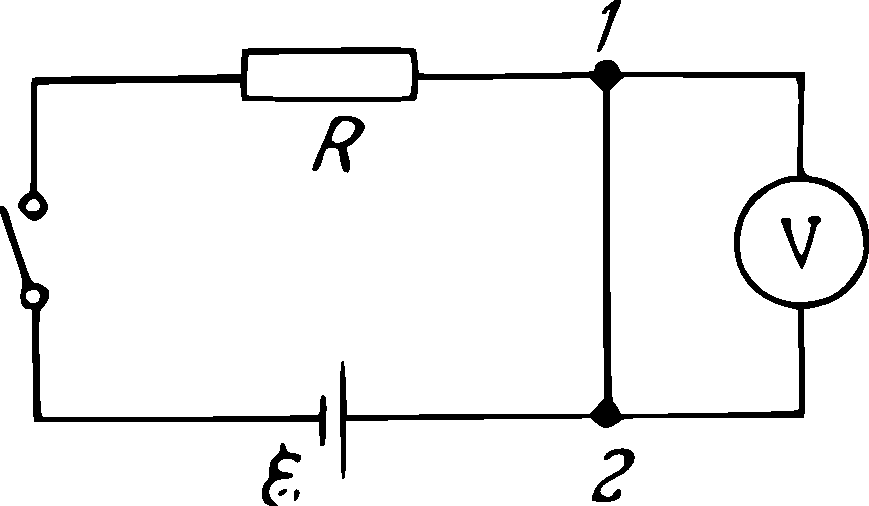
\includegraphics[width=0.85\textwidth]{figs/ch-21/fig-21-03.pdf}
\sidecaption{Generalized Ohm's law for a portion of the voltmeter circuit.\zhcap{电压表电路某段的广义欧姆定律。}\label{fig-21-03}}
\end{marginfigure}


\subsection{}\label{21.2.6} In a d.c. electric circuit with fixed conductors, the work done by the extraneous forces is completely consumed in heating the conductors \ssect{20.3.5}. The energy $E$, evolved in a circuit during the time $t$ throughout the whole volume of the conductor, is equal to
E - IUt,
where / is the current and U is the voltage. The quantity of heat $Q$ (\ssect{9.2.1}) in calories, cor­ responding to this energy and evolved in the conductor, is
\zhpar{在含有固定导体的直流电路中，非静电力所做的功完全用于使导体发热（见\ssect{20.3.5}）。在时间 $t$ 内，电路中整个导体体积里放出的能量 $E$ 等于}
\begin{equation*}
E = I U\,t,
\end{equation*}
where $I$ is the current and $U$ is the voltage. The quantity of heat $Q$ \ssect{9.2.1} in calories, corresponding to this energy and evolved in the conductor, is
\zhpar{式中 $I$ 为电流，$U$ 为电压。与该能量对应、在导体中放出的热量 $Q$（见\ssect{9.2.1}，以卡计）为}
\begin{equation*}
Q = 0.24 \, I U\,t.
\end{equation*}
All the other quantities are expressed in SI units (Appendix I). The \redem{Joule-Lenz} law states that the quantity of heat generated by current in a conductor is proportional to the current, voltage and time that the current flows. Other expressions of the Joule-Lenz law are:
\zhpar{其余各量均采用国际单位制（见附录 I）。\redem{焦耳-楞次定律}指出：导体中由电流产生的热量与电流、电压以及电流通过的时间成正比。焦耳-楞次定律的其他表达式为}
\begin{equation*}
Q = 0.24 \, I^{2} R\,t = 0.24 \frac{U^{2}}{R}t.
\end{equation*}

\section{Kirchhoff's Laws}
\label{sec-21.3}
\zhtitle{基尔霍夫定律}


\subsection{}\label{21.3.1} The analysis of \redem{complex (branched) circuits} consists in finding the currents in the various portions of the circuit in accordance with their given resistances and applied emf's.
\zhpar{所谓分析\redem{复杂（支路）电路}，就是根据各段电路给定的电阻及所接电动势，求出各段电路中的电流。}


\subsection{}\label{21.3.2} A \redem{branch point}, or \redem{junction}, in a branched circuit, or network, is a point where there are more than two possible directions of the current (\figr{fig-21-04}).
\zhpar{在支路电路或网络中，若某点处电流的可能流向多于两个，则该点称为\redem{支路点}，或称\redem{节点}（见\figr{fig-21-04}）。}

\begin{marginfigure}
\centering
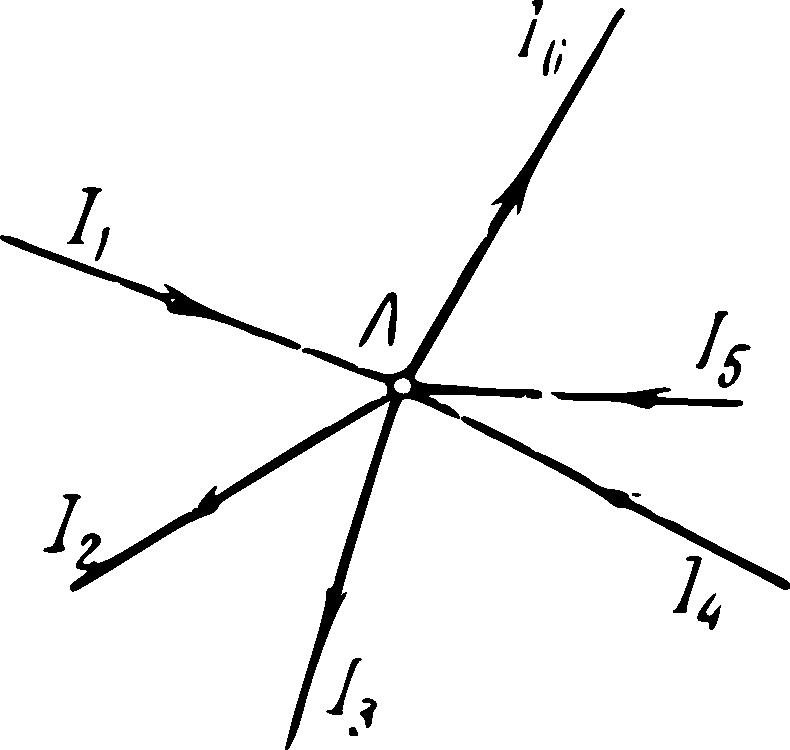
\includegraphics[width=0.75\textwidth]{figs/ch-21/fig-21-04.pdf}
\sidecaption{Analysing a branched circuit.\zhcap{分析支路电路。}\label{fig-21-04}}
\end{marginfigure}


\redem{Kirchhoff's first law} (point rule) states that the algebraic sum of the currents that meet at any junction of a network equals zero:
\zhpar{\redem{基尔霍夫第一定律}（节点电流定律）指出：网络中任一节点处汇聚的各电流的代数和为零：}
\begin{equation*}
\sum_{i =1}^{n} I_{i}= 0,
\end{equation*}
where $n$ is the number of conductors joined at the branch point and $I_{i}$ is the current at the point. Currents flowing toward the branch point are considered positive; those flowing away are considered negative.
\zhpar{式中 $n$ 为与该支路点相连的导体数，$I_{i}$ 为该点处的电流。流向支路点的电流取正，背离支路点的电流取负。}

\redem{Kirchhoff's second law (mesh rule)} states that in any closed loop (mesh of a network), arbitrarily chosen in a branched circuit (network), the algebraic sum of the products of the currents $I_{i}$ by the resistances $R_{i}$ of the corresponding portions of the loop is equal to the algebraic sum of the emf's in the loop. Thus
\zhpar{\redem{基尔霍夫第二定律}（回路定律）指出：在支路电路（网络）中任意选取的闭合回路（网络的网孔）中，各段电流 $I_{i}$ 与相应段电阻 $R_{i}$ 的乘积的代数和，等于该回路中各电动势的代数和。即有}
\begin{equation*}
\sum_{i =1}^{n_{1}} I_{i} R_{i}= \sum_{i =1}^{n_{1}} \emf_{i}
\end{equation*}
where $n_{1}$ the number of portions into which the loop is divided by branch points (junctions). In applying the mesh rule, a definite direction around the loop is chosen (either clockwise or counter­ clockwise). Currents coinciding in direction with the chosen one are considered positive. The emf's of the sources of electrical energy are considered positive if they produce currents whose direction coincides with the chosen one.
\zhpar{式中 $n_{1}$ 为回路被支路点（节点）分成的段数。应用回路定律时，须沿回路选定一个绕行方向（顺时针或逆时针）。与所选绕行方向一致的电流取正。若电源产生的电流方向与所选绕行方向一致，则该电源的电动势取正。}

\subsection{}\label{21.3.3} The following procedure is employed to analyse a complex (branched) d.c. circuit:
\zhpar{分析复杂（支路）直流电路的步骤如下：}
\begin{enumerate}[label = (\alph*)]
\item The directions of the currents are arbitrarily assigned in all the portions of the circuit.
\zhpar{任意指定电路各段中电流的方向。}
\item For $m$ branch points (junctions), $m - 1$ independent equations are written on the basis of Kirchhoff's first law.
\zhpar{对于 $m$ 个支路点（节点），依据基尔霍夫第一定律可列出 $m - 1$ 个独立方程。}
\item Arbitrary closed loops are separated out and, alter choosing the direction for going around each loop, a system of equations is written on the basis of Kirchhoff's second law. In a branched circuit consisting of $p$ portions (branches) between adjacent branch points and $m$ branch points (junctions), the number of independent equations based on the mesh rule equals $p - m + 1$. In selecting the loop, it is necessary for each new loop to contain at least one portion (branch) not included in the previously considered loops.
\zhpar{任意划分闭合回路，选定每个回路的绕行方向后，依据基尔霍夫第二定律列出方程组。在由相邻支路点之间的 $p$ 段（支路）和 $m$ 个支路点（节点）组成的支路电路中，依据回路定律所得的独立方程数为 $p - m + 1$。选取回路时，每个新回路至少应包含一段在先前已考虑的回路中未出现过的支路。}
\end{enumerate}

\subsection{}\label{21.3.4} To \redem{shunt an ammeter} means to connect an additional resistor $R_{sh}$, in parallel to the ammeter. This is done so that the ammeter, having the resistance $R_{0}$ and designed to measure a maximum current of $I_{0}$, can be applied to measure currents $I$ that exceed current $I_{0}$ (\figr{fig-21-05}). The required resistance of the shunt is found according to Kirchhoff's laws: $I = I_{0} + I_{sh}$ and $I_{0}R_{0} = I_{sh}R_{sh}$ from which $R_{sh}$ is eliminated:
\zhpar{所谓\redem{对电流表进行分流}，是指在电流表上并联一个附加电阻 $R_{sh}$。这样，内阻为 $R_{0}$、设计用来测量最大电流 $I_{0}$ 的电流表，便可用于测量超过 $I_{0}$ 的电流 $I$（见\figr{fig-21-05}）。所需分流电阻可由基尔霍夫定律求得：$I = I_{0} + I_{sh}$ 及 $I_{0}R_{0} = I_{sh}R_{sh}$，由这两式消去 $I_{sh}$ 后得到：}
\begin{equation*}
R_{sh} = \frac{I_{0}R_{0}}{I - I_{0}}
\end{equation*}
\begin{marginfigure}
\centering
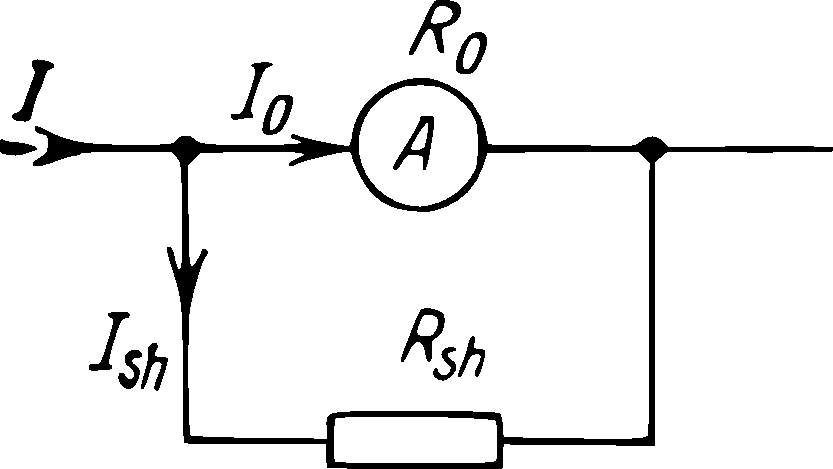
\includegraphics[width=0.75\textwidth]{figs/ch-21/fig-21-05.pdf}
\sidecaption{Analysing shunting of ammeter.\zhcap{分析电流表的分流。}\label{fig-21-05}}
\end{marginfigure}

\subsection{}\label{21.3.5} A potential difference $V_{1} - V_{2}= U$ across a portion of a circuit is to be measured by a voltmeter designed for a maximum measurement of $U_{0}$ volts \ssect{21.2.5} at a maximum permissible current of $I_{0}$ (with $U_{0} = I_{0}R_{0}$)and this potential difference exceeds $U_{0}$ (i.e. $U > U_{0}$). This can be done by connecting an additional \redem{resistor} $R_{a}$ in series with the voltmeter (\figr{fig-21-06}). The required additional resistance is determined from the equation $U = (R_{0}+ R_{a})I_{0}$, from which
\zhpar{若要测量电路某段两端的电势差 $V_{1} - V_{2}= U$，而电压表的最大量程为 $U_{0}$ 伏（见\ssect{21.2.5}），最大允许电流为 $I_{0}$（其中 $U_{0} = I_{0}R_{0}$），且待测电势差超过 $U_{0}$（即 $U > U_{0}$），则可在电压表上串联一个附加\redem{电阻器} $R_{a}$（见\figr{fig-21-06}）。由方程 $U = (R_{0}+ R_{a})I_{0}$ 确定所需附加电阻，即}
\begin{equation*}
R_{a} = \frac{U}{I_{0}} - R_{0}
\end{equation*}

\begin{figure}[h]%[-1cm]
\centering
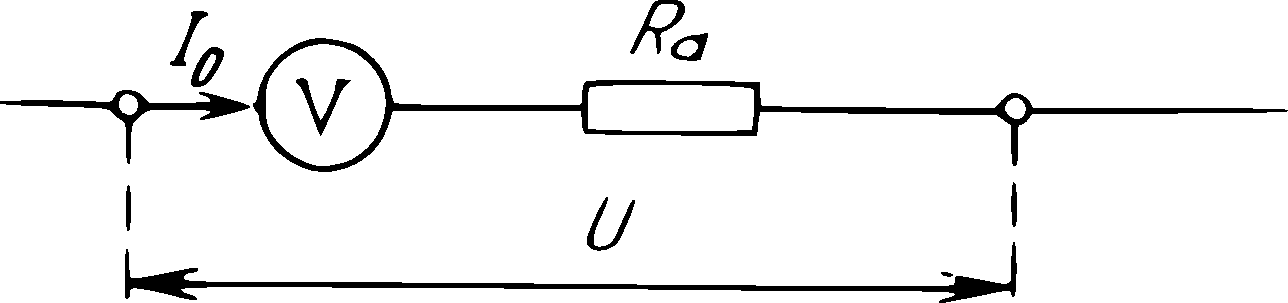
\includegraphics[width=0.75\textwidth]{figs/ch-21/fig-21-06.pdf}
\sidecaption{Additional resistor for a voltmeter.\zhcap{电压表的附加电阻。}\label{fig-21-06}}
\end{figure}